\setchapterpreamble[u]{\margintoc}

\chapter{Droplet Generation in Corrugated Ligaments}
\labch{breakup}


Ligaments constitute the penultimate stage in the complex sequence 
of capillary-driven topological changes that are 
typical of liquid fragmentation processes, 
finally resulting in the generation of polydisperse collections of drops. 
As we have seen in the previous chapter, there are several hypotheses 
in existing literature \sidecite{vill_1} 
that attempt to model the underlying physical mechanisms 
that are responsible for the selection of droplet size. 
A model first proposed by Villermaux and collaborators \sidecite{vill_2,vill_4}
asserts that the variance in the droplet sizes is strongly 
correlated to the initially corrugated shape of the 
ligament, from which the drops originate. 
These studies essentially demonstrate that the degree of polydispersity 
in the drop sizes can quite simply, be explained by considering the 
geometric shape of the ligaments, irrepective of the sequence of 
complicated fragmentation processes that gave rise to them in the first place.  


\begin{marginfigure}[4cm]
\centering
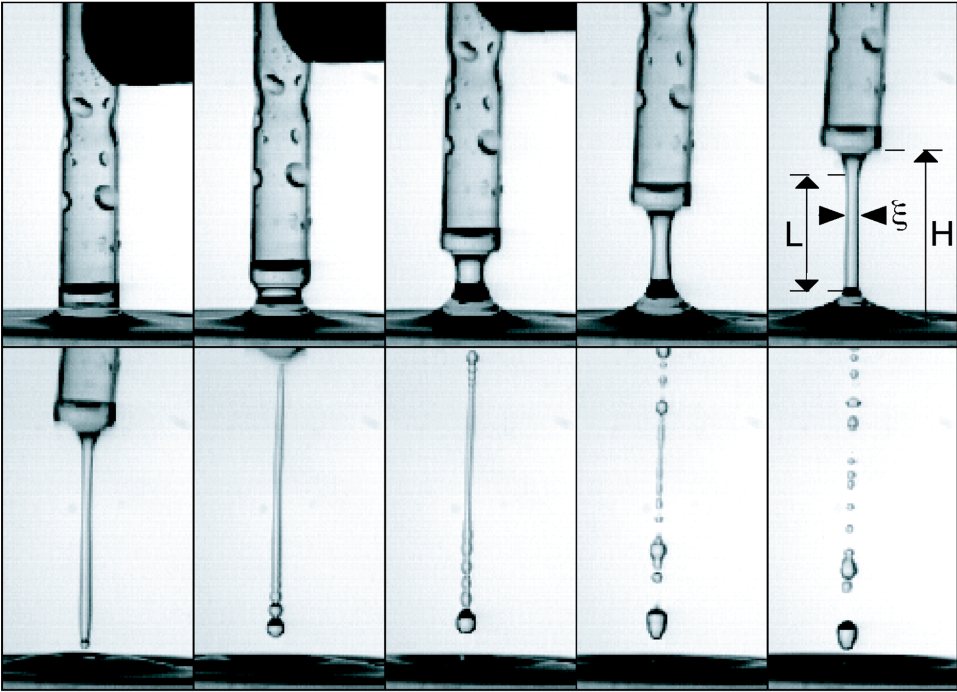
\includegraphics{plots/ligament_breakup/lig_mar_vill_pof04.png}
\caption{Fragmentation of stretched liquid (Newtonian) ligaments, reproduced 
	from Marmottant \& Villermaux \cite{vill_3}.
       	The complex rearrangement of the liquid volumes 
	inside the ligament results in its disintegration 
	into droplet of various sizes. 
	}
\end{marginfigure}

\marginnote{
The corrugation-coalescence mechanisn has been 
popularized in several studies such as \cite{vill_3,vill_1,vill_5,vill_6,vill_7},
and more recently in \cite{bonn,mckinley}.
}

In the context of the present body of work, we shall 
only concern ourselves with the dynamics of Newtonian fluids, 
described by the Navier-Stokes equations at the incompressible
and isothermal limits. 
The rearrangement of the liquid volumes that constitute
the ligaments play a key role in determining the size 
of the droplets that emerge immediately after the disintegration
of the ligament structure.  
The dynamics of these rearrangements prior to breakup are 
governed by non-linear interactions between several 
physical mechanisms such as the propagation of capillary waves
along the ligament surface, remnants of the internal flow, 
stretching induced by either the surrounding 
gas flow or acceleration into the surrounding medium itself,
and the dissipative effects of viscosity.  


%Due to the complex nature of such fragmentation processes, 
%it has proven to be quite a difficult challenge for both 
%experimental and numerical studies to establish the 
%mechanistic link between the initial surface corrugations 
%and the resulting drop size distributions.  
%
%
%In the present study, we have developed a numerical experiment 
%that grants us precise control over both quantitative and 
%qualitative aspects of such random corrugations, and its subsequent 
%influence on the resulting droplet sizes. 



\section{Breakup Regimes}

% Brief review, eggers , Keller-Miksis and Viscous regimes


%---------------------------------------------------------------
\section{Numerical Setup}
We perform direct numerical simulations of the two-phase 
Navier-Stokes equations under the incompressible framework. 
Material properties correspond to that of air-water systems at 20 degrees Celsius. 
Simulations are carried out in the axi-symmetric framework, 
therefore excluding the existence of azimuthal modes with 
respect to the central axis of the ligament. 

\paragraph{Platform : Basilisk}
\blindtext

\paragraph{Computational Schematic}
\blindtext

\paragraph{Random Surface Generation}
\blindtext

\paragraph{Parameterization}
\blindtext

\paragraph{Quantization of Waves}
\blindtext

%---------------------------------------------------------------

\section{Impact of Initial Conditions}

\paragraph{3D vs. 2D Simulations}
\blindtext

\paragraph{Effect of Spatial Resolution}
\blindtext

\paragraph{Effect of Droplet Removal}
\blindtext

\paragraph{Effect of Corrugation Amplitude}
\blindtext

\paragraph{Effect of Ohnesorge Number}
\blindtext

\paragraph{Effect of Cut-Off Wavenumber}
\blindtext

\paragraph{Effect of Aspect Ratio}
\blindtext


